%----------------------------------------------------------------------------------------------------------------------

\begin{frame}{Midcurve}

\begin{itemize}[noitemsep,label=\textbullet,topsep=2pt,parsep=2pt,partopsep=2pt]
\item Part is built by booleans of simpler swept volumes.
\item To generate Midsurface of a Swept volume
	\begin{itemize}[noitemsep,label=\textbullet,topsep=2pt,parsep=2pt,partopsep=2pt]
	\item Midcurves of the profile are calculated 
	\item swept similar to that of parent volume.
	\end{itemize}
	\vskip 3mm
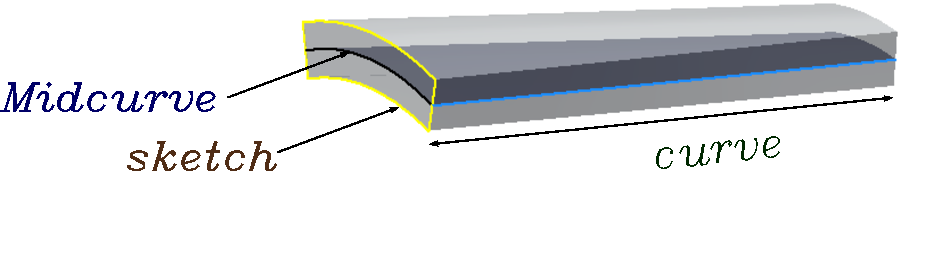
\includegraphics[width=0.85\linewidth]{../Common/images/MidsurfSmallProfile.pdf}
	\vskip -3mm
%\item 'Midcurve' is a skeleton of a 2D profile
%\item Simpler than the parent object
\item Useful in pattern recognition, approximation, similarity estimation, collision detection, animation, matching
\end{itemize}

%Notes: 

\end{frame}

%----------------------------------------------------------------------------------------------------------------------

\begin{frame}{How to compute Midcurve for following Shapes?}

\begin{itemize}[noitemsep,label=\textbullet,topsep=2pt,parsep=2pt,partopsep=2pt]%[label=,noitemsep,nolistsep]
\item[] 

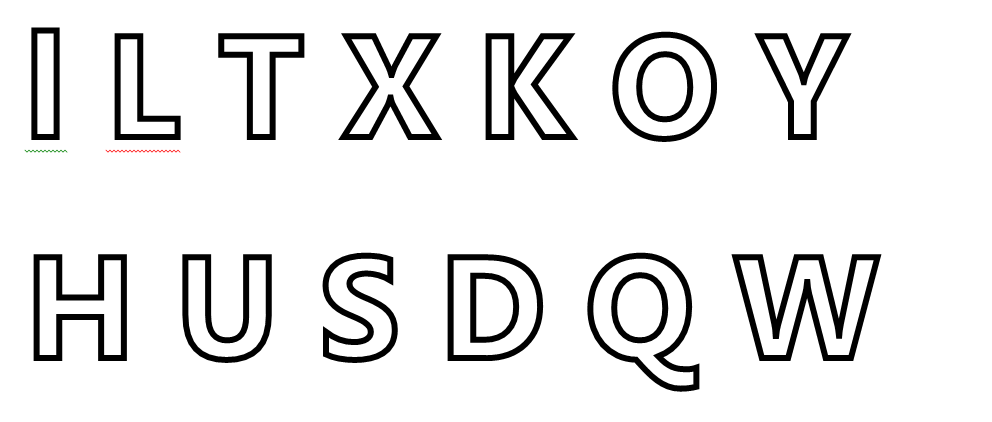
\includegraphics[width=0.8\linewidth]{../Common/images/Letters.png}


\item[] 
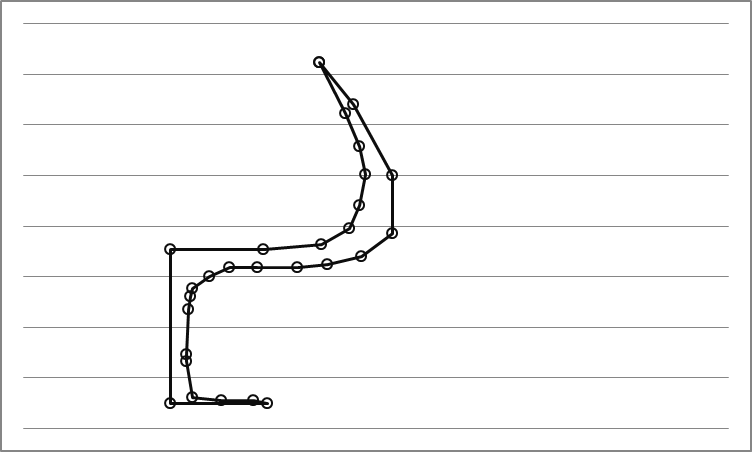
\includegraphics[width=0.4\linewidth]{../Common/images/Glasss.png}
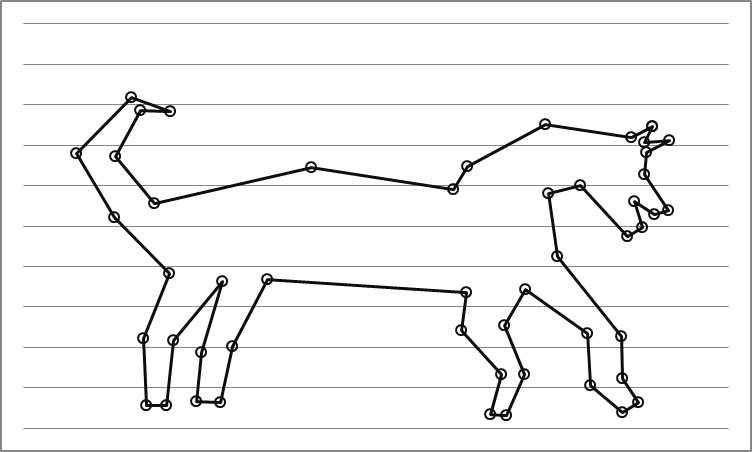
\includegraphics[width=0.4\linewidth]{../Common/images/Horses.png}

\item[] Any Idea?
\end{itemize}

%Notes: 

\end{frame}

%----------------------------------------------------------------------------------------------------------------------

\begin{frame}{Literature Survey}
\begin{itemize}[noitemsep,label=\textbullet,topsep=2pt,parsep=2pt,partopsep=2pt]
\item Started by Harry Blum in1967 \cite{Harry1967}
\item Rocha \cite{Rocha99} used both Decomposition and Skeletonization
\item For character recognition in images. 
\item From the results presented it appears that junctions like L, T were far from being well-connected.
\end{itemize}

%Notes: 

\end{frame}
%----------------------------------------------------------------------------------------------------------------------


\begin{frame}{Existing Methods}
\begin{tabular}{p{0.15\linewidth} p{.15\linewidth} p{.2\linewidth} p{.28\linewidth}}
\toprule
Method & Diagram & Description & Comments\\
\midrule
MAT \cite{Ramanathan2004} &  
\raisebox{-.9\height}{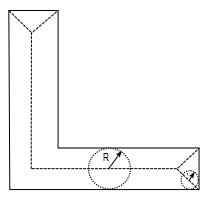
\includegraphics[width=0.9\linewidth]{../Common/images/MAT.png}} & 
Loci of centers of maximal disk & 
Computable for any shape. Unwanted branches.  \\ 

CAT \cite{Prasad2007} &  
\raisebox{-.9\height}{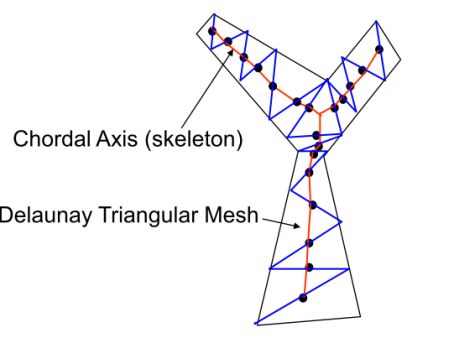
\includegraphics[width=0.9\linewidth]{../Common/images/CAT.png}} & 
Triangulation, then joins midpoints & 
Gaps towards end. Expensive triangulation.  \\ 

Straight Skeleton \cite{Henrik2004} &  
\raisebox{-.9\height}{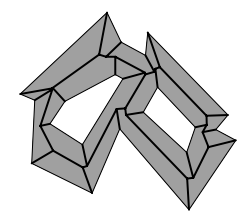
\includegraphics[width=0.9\linewidth]{../Common/images/Straight.png}}& 
Thinning from boundary.  & 
Unnecessary branches.\\
\bottomrule
\end{tabular}
\vspace{0.2in}

To overcome the weaknesses a novel algorithm is proposed...

\end{frame}
%----------------------------------------------------------------------------------------------------------------------
